\documentclass [10pt,letterpaper]{report}
%\documentclass[10pt,letterpaper]{article}
%\documentclass[10pt,letterpaper,twocolumn]{article}
%
%\documentclass[10pt,letterpaper,twocolumn]{report}
%\documentclass[10pt,letterpaper]{report}
%
%\usepackage[greek,english]{babel}
\usepackage[greek,english]{babel}
\usepackage[T1]{fontenc}
\usepackage{graphicx}
\usepackage{color}
\usepackage{wrapfig}


\textheight     =  8.4in
\textwidth      =  6.8in
%\parindent      =  0.0cm

\topmargin      =  -0.2in
\oddsidemargin  =  -0.2in
\evensidemargin =  -0.2in
%\hoffset        =  0.0cm
%\voffset        =  0.0cm

\newcommand{\nuSolve}{\greektext n\latintext Solve}
\newcommand{\thisVersion}{0.6.2}

\graphicspath{{graphics/}}

\begin{document}

\title{vgosDbMake-\thisVersion{}: User Guide}

\author{
Sergei Bolotin,
Karen Baver,
John Gipson,
David Gordon,
Daniel MacMillan
}

\date{\today}


\maketitle

\tableofcontents


\def\leftSp      {48mm}
\def\riteSp     {113mm}


\chapter{Introduction}
\label{intro}

This document describes how to use the utility vgosDbMake.

The software is designed to read fringe files, extract data from the files
and store it in vgosDb format.

The utility vgosDbMake is distributed in nusolve package that contains \nuSolve{}
software and utilities vgosDbMake, vgosDbCalc and vgosDbProcLogs. Each of the
utilities has its own version number that can differ from distribution version,
e.g., the first release of vgosDbMake-0.0.1 appeared in nusolve-0.2.10 package.

The guide covers \thisVersion{} version of the software. Since the vgosDbMake
is a simple utility we do not expect large modifications of the User Guide version
from version.


\section{Requirements}
\label{intro_reqs}

See \emph{\nuSolve{} User Guide} for the requirements.


\section{Changes from previous versions}
\label{intro_changes}

This section was added in 0.5.0 version of the nusolve distribution (version 0.3.0
of the vgosDbMake user guide). It covers changes in the software and the user guide.


\subsection{Changes in version 0.6.3}
vgosDbMake only treats as Mk4 root files those files whose names match the HOPS
specifications, other files are ignored. To override this feature a command line
option <<-g>> is added.

Extraction of channel bandwidth from fourfit files was added to the software.

\subsection{Changes in version 0.6.2}
The section \emph{\ref{config_paths} Setting paths to data} was updated to reflect
changes in master file handling.

\subsection{Changes in version 0.6.1}
Nothing essential was changed.

\subsection{Changes in version 0.6.0}
Support of version 2 of masterfile and new database naming convention is added.
See the chapter \emph{\ref{chapter_invokation} Invoking vgosDbMake} for details.


\subsection{Changes in version 0.5.6}
Nothing essential was changed.


\subsection{Changes in version 0.5.5}
Nothing essential was changed. Some corrections were made: If a correlator name is not
found in a masterfile and is not specified with "-r" option, the utility will use
analysis center abbreviated ID as a correlator name to prevent problems with creation
of Head.nc file. The regular expression for a valid source name in the map for sources
was modified: a dot was added as a valid char in a source name.


\subsection{Changes in version 0.5.4}
The command line arguments parser has switched to ARGP from GNU C Library.

Processing of correlator name was reworked. If it is available from VEX
files and not "difx" or "sfxc", the software will use it. Otherwise, it will
use correlator name from a masterfile. A user can override the correlator
name with "-r" option. Previously, this option worked only in combination
with an alternative database name (option "-d").


\subsection{Changes in version 0.5.3}
The software checks for duplicate scan names and corrects them if found. Also, it
checks for NaN in single band delays, group delays, delay rates, etc. and skips such
observations (sometimes it happens with KOMB files).

For KOMB files input vgosDbMake is able to correct group delays and rates for
reference station clock offset if a user provides a command line option "-x".
Chapter \emph{\ref{chapter_invokation} Invoking vgosDbMake} was modified to reflect
the change.


\subsection{Changes in version 0.5.2}
Nothing essential was changed.


\subsection{Changes in version 0.5.1}
Nothing essential was changed.



\subsection{Changes in version 0.5.0}
New command line arguments were added, see the chapter
\emph{\ref{chapter_invokation} Invoking vgosDbMake} for details.

A dry mode has been implemented, the software reads input files, creates and fills
all internal structures, but nothing is written.

Dealing with locale has been altered. Unfortunately, people do not read the manuals,
as a result their locale set up conflicts with HOPS parsing of fringe files. Now,
by default the locale is set to "C" after the utility is started. There are options
to configure this feature in the wizard as well as a command line argument.


\subsection{Changes in version 0.4.4}
A bug in creation vgosDb files has been fixed: values of the geocentric group delays and
the geocentric rates were swapped in the netCDF file "CorrInfo-difx\_b?.nc". Software
that use these data should check an attribute "Program", if it contains "vgosDbMake-0.4.3"
or earlier versions, the values of the geocentric group delays and the geocentric rates
need to swapped back. The bug was reported by Minghui Xu from Shanghai Observatory, China
(thanks!).

Processing of observations with non-empty error codes has been altered. The previous
versions discarded all data that have non-empty fringe error codes (which mimics
{\it dbedit} behavior). Starting with version 0.4.4 of vgosDbMake observations with
all fringe error codes are accepted. In addition, the command line option {\tt -e} is
added, see
the chapter \emph{\ref{chapter_invokation} Invoking vgosDbMake} for details.

\subsection{Changes in version 0.4.3}
This update contains bug fixes.

\subsection{Changes in version 0.4.2}
In this version behavior of vgosDbMake has been modified: if the environment
variable <<\$DISPLAY>> is not set, calls to pop up windows with error messages are
suppressed. Also, during creation of the wrapper file name, the attribute
<<\_i[Institution]>> will be added. To suppress the last option, the short
abbreviation of the affiliation should not be set (e.g., on the Fig.~\ref{fig-wizzard-3}
put an empty string instead of <<GSFC>>).

A warning about permanently increase of the log file size was added to the section
\emph{\ref{config_logger} Setting options of the logger}.


\subsection{Changes in version 0.4.1}
The command line options {\tt -p} and {\tt -W} are added in this version, see
the chapter \emph{\ref{chapter_invokation} Invoking vgosDbMake}.

A section \emph{\ref{sect_systemwide_settings} Using system-wide settings} is added.

The URL of software distribution has been updated in the chapter
\emph{\ref{chapt_concluding_remark} Concluding remark}.


\subsection{Changes in version 0.4.0}
The software has been modified to read fringe files that have new naming convention.

A new option was introduced: mapping non-standard names of stations and sources.
vgosDbMake can replace a non-standard station or source name with its conventional
counterpart. This feature is described in the chapter \emph{\ref{chapter_invokation}
Invoking vgosDbMake}.


\subsection{Changes in version 0.3.0}
The utility is able to read an alternative version of master files. The
use of the local master files is described in the section
\emph{\ref{config_paths} Setting paths to data}.

A notion about locale configuration of the shell environment have been
added to the chapter \emph{\ref{chapter_invokation} Invoking vgosDbMake}.

The sections \emph{\ref{intro_reqs} Requirements} and
\emph{\ref{intro_changes} Changes from previous versions} were added to
the chapter \emph{\ref{intro} Introductions}.







%%%%%%%%%%%%%%%%%%%%%%%%%%%%%%%%%%%%%%%%%%%%%%%%%%%%%%%%%%%%%%%%%%%%%%%%%%%%%%
%
%
\chapter{Installation}


The source codes of vgosDbMake is distributed along with \nuSolve{}
software. The latest stable version of the software one can find at
{\tt https://sourceforge.net/projects/nusolve} with a name like
{\tt nusolve-1.2.3.tar.gz}. Since the software is still in an active
development phase, we recommend you use the latest version.

Before installing the software you should check for three external
packages which vgosDbMake depends on. The Qt library provides the
graphical user interface. The netCDF library deals with I/O operations
in Common Data Form format. The Haystack Observatory Postprocessing
System, HOPS, is necessary to read fringe files.

Practically, all modern Linux distributions contain first two libraries.
There is a good chance that Qt library is already installed on your
computer (check your package manager or ask a system administrator). If,
for some reason, you cannot or do not want to install these packages
system-wide, you can download the sources and and install them in your
home directory. In this case (also, if the system installation put the
library(ies) in non-standard places) you will need to provide paths to
include files and libraries to the configure script.

The HOPS software should be installed manually, it is available from
the ftp site of Haystack Observatory, {\tt ftp://gemini.haystack.mit.edu/pub/hops}.

The first step in installing vgosDbMake is to extract the files in a
temporary directory and cd to it. Run a configure script in the root
directory of the package:
\begin{verbatim}
> ./configure <options>
\end{verbatim}
\noindent
Where a list of options of the configure script can be retrieved issuing

\begin{verbatim}
> ./configure --help
\end{verbatim}
\noindent
Several options are worth mentioning here. The place where to install
the software:
\begin{verbatim}
    --prefix=[PREFIX]
\end{verbatim}
\noindent
By default, it is {\tt /usr/local}. If you do not have permissions to
write there (which is a sign of a properly configured system), a user
can install the software into his/her home or somewhere else. In this
case, it is useful to add {\tt PREFIX/bin} to your {\tt PATH}
environment variable. Also, you may need to add {\tt PREFIX/lib} to your
{\tt LD\_LIBRARY\_PATH} variable.

Another option
\begin{verbatim}
    --with-qt-dir=[PATH_TO_QT-4.8]
\end{verbatim}
specifies where to look for Qt's files. The software is designed to work with
Qt library of version 4.8.7, using older or newer versions of the library
require modifying of the software sources or even change of its design.
Qt library itself is a rapid developing product, so to get rid of versions
race one can install a separate copy of Qt-4.8.7. In this case a directory
where the library was installed will be an argument of {\tt --with-qt-dir}
option.

Some Linux distributions put Qt's files in a non-standard way. In this case
the option splits into the two separate options:
\begin{verbatim}
    --with-qt-include =[PATH_TO_QT-4.8 includes]
    --with-qt-lib     =[PATH_TO_QT-4.8 libraries]
\end{verbatim}
Where the first one specifies where to search for include files and the last
one is for library files.

To point out on non-standard places of netCDF files, use the following options:
\begin{verbatim}
    --with-netcdf-include =[PATH_TO_NETCDF includes]
    --with-netcdf-lib     =[PATH_TO_NETCDF libraries]
\end{verbatim}
to specify where the include file and the libraries are.

To trigger on the compilation of vgosDbMake, the configure script expects one
of the following options:
\begin{verbatim}
    --with-hops-dir=[PATH_TO_HOPS]
\end{verbatim}
or
\begin{verbatim}
    --with-hops-include=[PATH_TO_HOPS include files]
    --with-hops-lib=[PATH_TO_HOPS libraries]
    --with-hops-share=[PATH_TO_HOPS shared data]
\end{verbatim}
Even if your HOPS library was configured with {\tt -{}-prefix=/usr/local} and all
files are in standard places, you need to provide the option {\tt -{}-with-hops-dir=/usr/local}
to turn on compiling vgosDbMake utility.

Another option, {\tt -{}-enable-vgosDbMake-only}, removes \nuSolve{} and other
utilities but vgosDbMake from the list of software that should be build and
installed. If you want to install only vgosDbMake utility, you need to
invoke {\tt configure} script as follow:
\begin{verbatim}
> ./configure --prefix=[...] --with-hops-dir=[PATH_TO_HOPS] --enable-vgosDbMake-only [other options]
\end{verbatim}
Note, the option {\tt --with-hops-dir=} is still necessary to turn on building
of vgosDbMake.


In the file {\tt INSTALL.local} in the root of the distributive tree one can
find details about specifying configure's options to assemble the software
with Qt and netCDF libraries.

If the {\tt configure} script finished without errors, type the
following commands:
\begin{verbatim}
> make
> make install
\end{verbatim}
\noindent
and the software will be installed in the {\tt PREFIX} directory. The
command {\tt make check} is optional, it is a placeholder for checking
suite that will be developed later.





%%%%%%%%%%%%%%%%%%%%%%%%%%%%%%%%%%%%%%%%%%%%%%%%%%%%%%%%%%%%%%%%%%%%%%%%%%%%%%
%
%
\chapter{Invoking vgosDbMake}
\label{chapter_invokation}
To invoke vgosDbMake type (specifying if necessary the full path
to the executable) program name and path where fringe files of a VLBI session are:
\begin{verbatim}
> vgosDbMake <PATH_TO_DATA>
\end{verbatim}
\noindent
The utility also accepts command line arguments. The arguments consist of
two groups of options and a name of alternative configuration. The first
group of options is related to Qt library and controls how the application
will appear and behave. See Qt documentation about details, (e.g.,
https://doc.qt.io/qt-5.14/qguiapplication.html).
%http://qt-project.org/doc/qt-4.8/qapplication.html\#QApplication).
The another group of options is used by itself. To get the list
of these arguments, type
\begin{verbatim}
> vgosDbMake --help
\end{verbatim}
\noindent
Here are command line arguments that are available at the time of writing:
\vspace{5mm}

\begin{tabular}{p{\leftSp}p{\riteSp}}
\multicolumn{2}{c}{General options:}\\

{\tt -f, -{}-mf-version=NUM}    & Set the expected masterfile format version to NUM. The possible format versions are 1 and 2.\\
{\tt -l, -{}-std-locale}        & Use the standard locale.\\
{\tt -o, -{}-output-dir=STRING} & Use an alternative path STRING to save files in vgosDb format.\\
\end{tabular}
\vspace{5mm}

\begin{tabular}{p{\leftSp}p{\riteSp}}
\multicolumn{2}{c}{Configuration control:}\\
{\tt -a, -{}-alt=STRING}        & Use an alternative configuration STRING.\\
\end{tabular}
\vspace{5mm}

\begin{tabular}{p{\leftSp}p{\riteSp}}
\multicolumn{2}{c}{Database edit options:}\\
{\tt -d, -{}-database=STRING}   & Set database name to STRING.\\
{\tt -r, -{}-correlator=STRING} & Set correlator name to STRING.\\
{\tt -s, -{}-exp-sn=NUM}        & Set experiment serial number to NUM.\\
\end{tabular}
\vspace{5mm}

\begin{tabular}{p{\leftSp}p{\riteSp}}
\multicolumn{2}{c}{Data extraction control:}\\
{\tt -e, -{}-exclude=CHAR}      & exclude observations with fringe error code CHAR. If CHAR is "*" only observations
    that have no fringe error code will be extracted. There can be more than one "-e" option, e.g.: -eA -eB.\\
{\tt -g, -{}-all-rootfile-names}& Assume root file names are in arbitrary form.\\
{\tt -m, -{}-map=STRING}        & Set a name map file to STRING.\\
{\tt -t, -{}-report=STRING}     & Set a correlator report file to STRING.\\
{\tt -x, -{}-adjust-ref-stn}    & KOMB files input only: adjust delays and rates for a reference station clock offset (experimental mode).\\
\end{tabular}
\vspace{5mm}

\begin{tabular}{p{\leftSp}p{\riteSp}}
\multicolumn{2}{c}{Invocation of startup wizard:}\\
{\tt -w, -{}-wizard}            & Force call of the startup wizard.\\
{\tt -W, -{}-sys-wide-wizard}   & Run startup wizard for the system-wide settings.\\
\end{tabular}
\vspace{5mm}

\begin{tabular}{p{\leftSp}p{\riteSp}}
\multicolumn{2}{c}{Operation modes:}\\
{\tt -?, -{}-help}              & Give this help list.\\
{\tt -p, -{}-print-setup}       & Print set up and exit.\\
{\tt -q, -{}-dry-mode}          & Process in a "dry run" mode: files will not be created, instead names of the files will be printed.\\
{\tt     -{}-usage}             & Give a short usage message.\\
{\tt -V, -{}-version}           & Print program version.\\
\end{tabular}
\vspace{5mm}


\noindent
Most of these options are used either to override the current software
configuration or for the debug purposes.

Starting with version 0.6.0, vgosDbMake can use version 2 format of masterfiles and create a database
with new naming convention. To specify what naming convention vgosDbMake should use, provide the 
option <<-f "NUM">>. Value of "NUM" can be either "1" (old naming convention) or "2" (new naming 
convention). For example, using
\begin{verbatim}
> vgosDbMake -f2 [...]
\end{verbatim}
will create a database using new naming convention. It is necessary that the corresponding masterfile
in the format of version 2 is exist in the proper directory 
(see Section \emph{\ref{config_paths} Setting paths to data}).
Masterfiles of old and new formats have different names and can co-exist in one directory.
If the option  <<-f "NUM">> is not provided, current version of vgosDbMake will use the
old format of a masterfile and old naming convention.

Reading Mk4 fringe files vgosDbMake assumes that names of input files comply to the HOPS
specifications. Starting with version 0.6.2 the software reads Mk4 root file only if its
name fits to pattern of an IVS source name and ignore all other files. To override this
option, use <<-g>> command line option.

The option <<-e "fringeErrorCode">> allows a user to filter out observations with the fringe error
code "fringeErrorCode". For example,
\begin{verbatim}
> vgosDbMake -eA [...]
\end{verbatim}
will exclude all observations that have the fringe error code "A". The options
<<-e>> can be stacked, e.g..
\begin{verbatim}
> vgosDbMake -eA -eB -eC -eD [...]
\end{verbatim}
will result in exclusion of observations with the fringe error codes "A" to "D".
A special case <<-e*>> suppress all observations with any non-empty fringe error
codes (that mimics how {\it dbedit} process observations).


The option <<-m>> specifies an ASCII file with station and source names map
that the software should use. This feature is designed to make possible to
alter a non-common station or source name that appears in fringe files to
its standard name. Also, it is possible to specify that an observation with
some specific station or source should not be included in a session. The format
of a map file is following:
\begin{verbatim}
stn:[input name] => [output name]
src:[input name] => [output name]
\end{verbatim}
\noindent
where <<[input name]>> is a name of a station or source as it appears in fringe
or KOMB files and <<[output name]>> is how it should be translated. A special value
for the output name <<-{}-{}->> means that the object should be skipped from the session.

For example, using a map file {\sl mapFile} of the following content:
\begin{verbatim}
#
#
# stations:
stn: VLBA_PT => PIETOWN
stn: VLBA_MK => MK-VLBA
stn: WETTDBBC => ---

# sources:
src: 0718+792 => 0718+793
src: 1228+126 => 3C274
src: 1637+826 => NGC6251
\end{verbatim}
\noindent
as
\begin{verbatim}
> vgosDbMake -m mapFile <path-to-fringe-files>
\end{verbatim}
\noindent
will override station names <<VLBA\_PT>> and <<VLBA\_MK>> as <<PIETOWN>> and
<<MK-VLBA>>, and exclude all observations on the station <<WETTDBBC>>. Also,
source names <<0718+792>>, <<1228+126>> and <<1637+826>> will have the following
names in the vgos database: <<0718+793>>, <<3C274>> and <<NGC6251>>.


The command line argument <<-l>> preserve altering of the locale. If you want to
use this option,
please check locale setting of your shell environment.
The HOPS software that parses VEX files uses libC functions that are locale
aware. Different languages have different rules for string comparison,
representation of integer and real numbers and so on, so using locale other
than standard "C", "POSIX" or "en" could cause incorrect work of the
software. You can check your environment locale setting with command
\begin{verbatim}
> locale
\end{verbatim}
\noindent
Consult with your system administrator for details.





%%%%%%%%%%%%%%%%%%%%%%%%%%%%%%%%%%%%%%%%%%%%%%%%%%%%%%%%%%%%%%%%%%%%%%%%%%%%%%
%
%
\chapter{Configuring the software}
When vgosDbMake is invoked the first time or new alternative
configuration name has been provided, it calls a setup wizard. The
wizard is a small application that asks a user few questions about the
configuration.

If you want to change your current configuration, run vgosDbMake with
{\tt -w} option:
\begin{verbatim}
> vgosDbMake -w
\end{verbatim}
\noindent
If you want to set up (or change) the configuration of alternative setup,
invoke vgosDbMake with {\tt -a AltCfg} option, e.g.:
\begin{verbatim}
> vgosDbMake -w -a IVS-R4
\end{verbatim}



\section{Using system-wide settings}
\label{sect_systemwide_settings}
On a system with several users it is useful to set up common software settings,
like path to observations, data files, and so on. To set up such settings, invoke
the utility with {\tt -W} option. Obviously, you have to have write access to the
directory with system-wide settings. By default, the system-wide settings directory
is derived from {\sl \$\{prefix\}} variable of the {\tt configure} script and is
set to {\sl \$\{prefix\}/etc/xdg}. It can be overwritten using {\sl --sysconfdir}
option of the {\tt configure} script.

The system-wide settings take an effect if user settings do not exist (e.g., first
run of the software), they do not change existing user's settings.

Combination of the option {\tt -W} with the option {\tt -a AltCfg} discards
using the system-wide settings, the setup wizard will use the alternative setup
instead.

Due to a problem in implementation of QSettings object, the system-wide settings
option is available only if you have Qt library of version 4.8.0 or newer.


\section{Setting paths to data}
\label{config_paths}
On the first after introduction wizard's page, "Home directory", user can
set up paths to the default directories. The home directory of vgosDbMake
is a place where all non-absolute paths refer to.

\begin{figure}[htb!]
  \begin{center}
    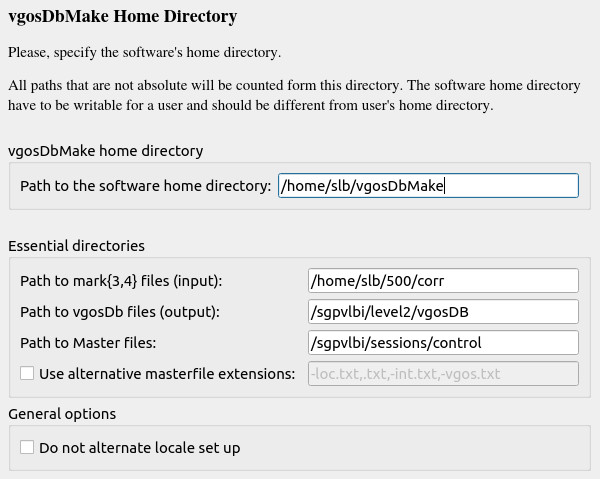
\includegraphics[width=0.6\textwidth]{wz-1.jpg}
  \end{center}
  \caption{Setting up paths.}
  \label{fig-wizzard-1}
\end{figure}

The path to input default locations of correlator files is in {\tt Path
to mark\{3-4\} files} filed. If you specify an argument that is not an
absolute path, vgosDbMake will search data counting from this directory.
For example, if the fringe files are in a directory {\tt
/home/slb/500/correlator/3449}, then, according to set up shown on
Fig.~\ref{fig-wizzard-1}, I can run vgosDbMake as
\begin{verbatim}
> vgosDbMake 3449
\end{verbatim}
Also, I can use absolute path and it will override the configuration:
\begin{verbatim}
> vgosDbMake /home/slb/500/correlator/3449
\end{verbatim}

The path to output directory is specified by the field {\tt Path to VgosDb files}.
A user can override it with {\tt -o} command line option. The data structure of
vgosDb files would looks like
\begin{verbatim}
   <VGOSDB_ROOT>/YYYY/YYMMMDDBL/<data files>
\end{verbatim}
Where {\tt VGOSDB\_ROOT} is a directory specified in the wizard, {\tt YYYY} is
a year and {\tt YYMMMDDBL} is a database name. For the example of vgosDbMake
invocation above and with standard master file, the output will be written
in the directory
\begin{verbatim}
   <VGOSDB_ROOT>/2015/15AUG03XA/
\end{verbatim}

The software uses master files to figure out proper database name. If a
session is not in master file, a user can specify the database name using
{\tt -d} command line option. The path to master files is a place where
master files suppose to be. You can obtain the files from
\begin{center}
{\tt
https://cddis.nasa.gov/archive/vlbi/ivscontrol/
}
\end{center}
\noindent
Time from time the files need to be updated. In addition to the standard master
files, a user can use its own "local" master file. The format of the local master
file should be the same as the standard one, its name have to be in the form
"masterYY-loc.txt", where "YY" -- two digits of the year. This feature is designed
for testing purposes or processing non-standard VLBI sessions. The software first
checks for the local master files, if it found a record there it stops the search,
so records in the canonical master files can be overwritten using the local
master file.

Starting with version 0.8.2 of the distribution, an option to expilictly set names
for master files is added. If a user sets the check box {\sl Use alternative
masterfile extensions} to <<on>>, then vgosDbMake will compose the masterfile names
using a provided list of extensions. The list is a set of strings separated by
comma (","), colon (":") or semicolon (";") char. The software adds the extension
from the list to the basic name, "masterYY" or "masterYYYY", and reads such a file.
The order of files lookup is corresponding to the order of masterfile
extensions in the list. The default list of masterfile extensions is
"-loc.txt,.txt,-int.txt,-vgos.txt".





The check box {\tt Do not alternate locale set up} controls how the utility
deals with locale set up. By default it is <<off>>.


\section{Setting user identities}
The second and third pages of the wizard, Fig.~\ref{fig-wizzard-2}-\ref{fig-wizzard-3},
set up user identities.

\begin{figure}[htb!]
  \begin{center}
    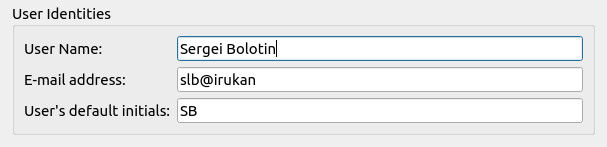
\includegraphics[width=0.6\textwidth]{wz-2.jpg}
  \end{center}
  \caption{Setting up user ID.}
  \label{fig-wizzard-2}
\end{figure}

%\section{Setting affiliation}

\begin{figure}[htb!]
  \begin{center}
    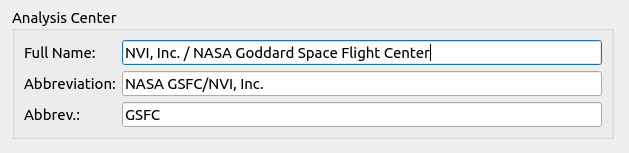
\includegraphics[width=0.6\textwidth]{wz-3.jpg}
  \end{center}
  \caption{Setting up affiliation.}
  \label{fig-wizzard-3}
\end{figure}

We strongly encourage users to provide, at least, a working e-mail
address.

Information collected by these two pages are used only for composing the
history part of vgosDb files and in vgosDbMake log file.

The short form of the abbreviated affiliation (<<Abbrev.>> on the
Fig.~\ref{fig-wizzard-3}) is used in wrapper file names as an attribute
{\sl \_i<Institution>}. If the field is empty, the attribute will not be
added to a name of a wrapper file.


\section{Setting options of the logger}
\label{config_logger}
The last page of the start up wizard, Fig.~\ref{fig-wizzard-4}, sets up
properties of the logging subsystem. The field {\tt Log file name} is
a name of a file where the log messages will be saved if the checkbox
{\tt Save log to the file} is checked <<on>>. The file will appear in
vgosDbMake home directory, Fig.~\ref{fig-wizzard-1}. The {\tt Log capacity}
is an amount of log records that are kept in internal structure before
send them to a file. The checkbox {\tt Put time stamps} turns on
adding time tags to the log messages.

\begin{figure}[htb!]
  \begin{center}
    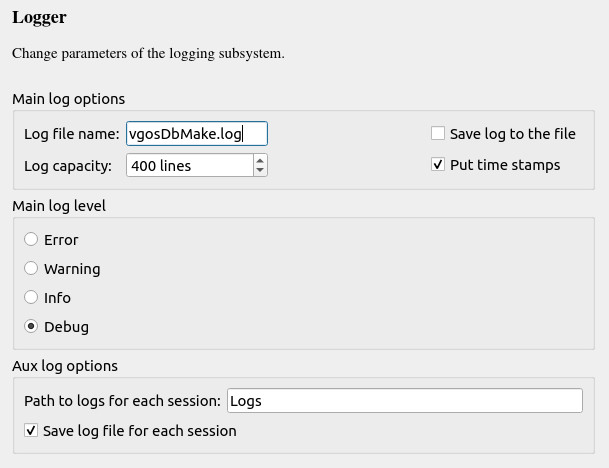
\includegraphics[width=0.6\textwidth]{wz-4.jpg}
  \end{center}
  \caption{Setting up logger.}
  \label{fig-wizzard-4}
\end{figure}

The {\tt Log level} determines how verbose the log output will be. The {\tt Debug}
level, as shown on the figure, could be useful for debugging purposes. For
routine operations the {\tt Info} level will be preferred.

%The software does not control the size of the main log file, it will grow up
%with each invocation of the utility. A user should control the size of the log
%file and remove or back it up, what is necessary.

Another log file will be created on a per session basis if the checkbox
{\tt Save log file for each session} is turned <<on>>. The aux log file
will be saved in {\tt Path to logs for each session} directory and its
name will be the same as the database name plus ".log" extension.

{\bf \color{red}WARNING}: If the logger is instructed to save data in
the log file, the size of the file will grow up. The software does not
check the size of the file (it does not know about your intentions), and
eventually the file could take all free space on your computer! If you
do not need the log output from previous runs, please, remove the file on
a regular basis.



%%%%%%%%%%%%%%%%%%%%%%%%%%%%%%%%%%%%%%%%%%%%%%%%%%%%%%%%%%%%%%%%%%%%%%%%%%%%%%
%
%
\chapter{Concluding remark}
\label{chapt_concluding_remark}
Currently, this document is in the developmental stage, its content could change
time from time. Check for new versions at the ftp site:

\begin{verbatim}
      https://sourceforge.net/projects/nusolve
\end{verbatim}

\noindent
If you have questions or suggestions that will improve the software or
the User Guide, please e-mail us at:

\begin{verbatim}
      <mailto:sergei.bolotin@nasa.gov>
\end{verbatim}

%\noindent
%Happy !


%%%%%%%%%%%%%%%%%%%%%%%%%%%%%%%%%%%%%%%%%%%%%%%%%%%%%%%%%%%%%%%%%%%%%%%%%%%%%%
%
%
\begin{thebibliography}{99}

\bibitem{Bolotin2010}
S. Bolotin, J. Gipson, D. MacMillan: ``Development of a New VLBI Data
Analysis Software". In: International VLBI Service for Geodesy and
Astrometry 2010 General Meeting Proceedings, edited by D. Behrend and K.
Baver, NASA/CP-2010-215864, 197-201, 2010.


\bibitem{Bolotin2011}
S. Bolotin, J. Gipson, D. Gordon, D. MacMillan: ``Current Status of
Development of New VLBI Data Analysis Software". In: Proceedings of the
20th Meeting of the European VLBI Group for Geodesy and Astrometry,
edited by W. Alef, S. Bernhart, A. Nothnagel, Schriftenreihe des
Instituts f\"ur Geod\"asie und Geoinformation der Universit\"at Bonn,
Nr. 22, ISSN 1864-1113, 86-88, 2011.


\bibitem{Bolotin2012}
S. Bolotin, K. Baver, J. Gipson, D. Gordon, D. MacMillan: ``The First
Release of $\nu$Solve". In: International VLBI Service for Geodesy and
Astrometry 2012 General Meeting Proceedings `Launching the
Next-Generation IVS Network', edited by D. Behrend and K. Baver,
NASA/CP-2012-217504, 222-226, 2012.


\end{thebibliography}


\end{document}


